\documentclass[]{article}
\usepackage{lmodern}
\usepackage{setspace}
\setstretch{1.5}
\usepackage{amssymb,amsmath}
\usepackage{ifxetex,ifluatex}
\usepackage{fixltx2e} % provides \textsubscript
\ifnum 0\ifxetex 1\fi\ifluatex 1\fi=0 % if pdftex
  \usepackage[T1]{fontenc}
  \usepackage[utf8]{inputenc}
\else % if luatex or xelatex
  \ifxetex
    \usepackage{mathspec}
    \usepackage{xltxtra,xunicode}
  \else
    \usepackage{fontspec}
  \fi
  \defaultfontfeatures{Mapping=tex-text,Scale=MatchLowercase}
  \newcommand{\euro}{€}
\fi
% use upquote if available, for straight quotes in verbatim environments
\IfFileExists{upquote.sty}{\usepackage{upquote}}{}
% use microtype if available
\IfFileExists{microtype.sty}{%
\usepackage{microtype}
\UseMicrotypeSet[protrusion]{basicmath} % disable protrusion for tt fonts
}{}
\usepackage[margin=1in]{geometry}
\ifxetex
  \usepackage[setpagesize=false, % page size defined by xetex
              unicode=false, % unicode breaks when used with xetex
              xetex]{hyperref}
\else
  \usepackage[unicode=true]{hyperref}
\fi
\hypersetup{breaklinks=true,
            bookmarks=true,
            pdfauthor={Christopher Gandrud, Sahil Deo, Christian Franz, and Mark Hallerberg},
            pdftitle={Measuring Real-time Perceptions of Financial Market Stress},
            colorlinks=true,
            citecolor=blue,
            urlcolor=blue,
            linkcolor=magenta,
            pdfborder={0 0 0}}
\urlstyle{same}  % don't use monospace font for urls
\setlength{\parindent}{0pt}
\setlength{\parskip}{6pt plus 2pt minus 1pt}
\setlength{\emergencystretch}{3em}  % prevent overfull lines
\setcounter{secnumdepth}{5}

%%% Use protect on footnotes to avoid problems with footnotes in titles
\let\rmarkdownfootnote\footnote%
\def\footnote{\protect\rmarkdownfootnote}

%%% Change title format to be more compact
\usepackage{titling}

% Create subtitle command for use in maketitle
\newcommand{\subtitle}[1]{
  \posttitle{
    \begin{center}\large#1\end{center}
    }
}

\setlength{\droptitle}{-2em}
  \title{Measuring Real-time Perceptions of Financial Market Stress}
  \pretitle{\vspace{\droptitle}\centering\huge}
  \posttitle{\par}
  \author{Christopher Gandrud, Sahil Deo, Christian Franz, and Mark Hallerberg}
  \preauthor{\centering\large\emph}
  \postauthor{\par}
  \date{}
  \predate{}\postdate{}

\usepackage{graphicx}
\usepackage{bm}


\begin{document}

\maketitle


\textbf{Note: This work is in the early stages of development. It will
be updated significantly.}\footnote{Please contact Christopher Gandrud
  (\href{mailto:gandrud@hertie-school.org}{\nolinkurl{gandrud@hertie-school.org}}).
  Thank you to Ronen Palan for helpful comments. All data and
  replication material can be found at:
  \url{https://github.com/christophergandrud/EIUCrisesMeasure}.}

\begin{abstract}
A wide range of political economy research on the causes, responses to, and effects of banking crisis needs an accurate and reliable measure of banking crises that is comparable across countries and ideally includes information on crisis severity. Most research to date uses one of two series of crisis data: Reinhart and Rogoff (2009) or Laeven and Valencia (2013). These measures are lacking in that they are simple dichotomous indicators of financial crisis and differ considerably in their start and end dates for many incidents. They are also constructed after the fact and so tend to be biased towards severe crises and away from those where government responses effectively calmed emerging trouble. Recent efforts, namely Jing et al. (2015), Rosas (2009), and Romer and Romer (2015) have attempted to develop more reliable measures of crises that also include continuous information on severity. Each of these approaches have important shortcomings. Jing et al.’s measure is based on central bank’s policy responses, which researchers may want to examine as a dependent variable. Rosas relies on nationally reported banking system data, but as Copelovitch, Gandrud, and Hallerberg (2015) show the reporting of this data is often endogenous to financial system difficulties [MAYBE CHANGE]. Romer and Romer’s approach relies on very time intensive human coding of texts from the OECD and aggregates these codings using a simple summation method. Their approach, though it avoids the issues present in Jing et al. (2015) and Rosas (2009), is very laborious to construct, subjective, and equally weights each item in their coding scheme, which may not be reasonable. This paper describes the motivation and construction of our new measure of real-time perceptions of financial market stress based on kernel principal component analysis (PCA) of Economist Intelligence Unit monthly country reports. We refer to this measure as the EIU Perceptions of Financial Market Stress (EPFMS) Index. In doing so, we not only develop a novel indicator of financial market stress, but we also make a contribution to the wider political science literature by demonstrating how kernel PCA can be used to summarize vast quantities of qualitative texts into useful cross-sectional time-series indicators.
\end{abstract}

Why and how do politicians respond to financial market stress? This
question has attracted considerable attention recently following the
2007-2009 financial crisis and earlier following the late-1990s Asian
financial crisis. However, virtually all of this research lacks a
crucial variable: a real-time indication of the level of financial
market stress that policy-makers believed that they faced. To understand
why politicians made a given policy choice, we need to have a measure
the conditions that they believed they were responding to.

Most research has used \emph{post-hoc} assessments of banking crisis as
a second-best alternative. However, this presents clear problems.
Chiefly, using such measures creates clear selection bias as stress that
politicians responded to effectively will not be selected. In addition,
these measures are typically binary and so give no indication of stress
intensity. The measures are also at gross intervals, typically yearly,
prohibiting sub-annual analysis.

In this paper we aim to overcome these problems by develop a new index
of real-time perceptions of financial market stress. The Index is
created using a kernel principal component analysis (PCA) of monthly
Economist Intelligence Unit (EIU) reports. We it the EIU Perceptions of
Financial Market Stress (EPFMS) Index. This measure should supplant
previous second-best measures of financial market stress by researchers
aiming to understand why and how policy-makers respond to financial
crisis. In so doing, we make a contribution to the wider political
science literature by showing how kernel PCA can be used to summarize
vast quantities of qualitative texts into cross-sectional time-series
indicators.

We start the paper by detailing our motivation for creating a real-time
index of perceptions of financial market stress. We then discuss the
construction of the Index and compare it to widely used previous
measures of financial market stress. {[}WOULD BE NICE TO HAVE A
REPLICATION OF AN IMPORTANT PAPER{]}.

\section{Motivation}\label{motivation}

Researchers have tended to rely on two data sources for cross-country
information on when a country is facing a financial crisis: Laeven and
Valencia (2013) and Reinhart and Rogoff (2009). Knowing when crises
started (and when they have ended) is crucial for research trying to
understand issues such as how crises affect economic output, how
governments choose to respond to financial market distress, and what the
fiscal costs of financial crises are.

There are a number of problems with these indicators. Unlike economic
recessions, financial crises are poorly defined in previous sources.
This contributes to large inconsistencies between the timing of crises
in the Laeven and Valencia (2013) and Reinhart and Rogoff (2009) data
sets (Chaudron and Haan 2014). For example, Japan is labeled as having a
crisis between 1997 and 2001 by the former, but 1992-1997 in the latter.
Gandrud and Hallerberg (2015) also find that there are significant
difference in crisis timing between different versions of the Laeven and
Valencia (2013) data. Crises are also identified by researchers who know
what happened. Financial market stress that is addressed well by
policymakers, preventing a major crisis, may therefore not be included.
Similarly, stress that is temporarily dampened through unsustainable
policy measures, only to flare up later, is not clearly recorded. This
makes it difficult to adequately study why and how politicians respond
to financial market stress. Related to this, current measures are
dichotomous thus errors have large consequences for creating bias when
used in econometric models. They also do not give any indication of how
severe a crisis is.

Overall, we lack the continuous real-time measure of financial market
stress that we need to be able to adequately examine why and how
policy-makers respond to financial market problems.

There have been a number of recent attempts to create crisis measures
that overcome these issues. Building on {Von Hagen} and Ho (2007), Jing
et al. (2015) developed am index of money market pressure based on
changes in short-term interest rates and stocks of central bank
reserves. However, this measure conflates distress and policy responses,
assuming central banks use the same reaction function to increased
demand for liquidity. Rosas (2009) developed a dynamic latent trait
model of banking system distress. However, his measure relies on
nationally reported data to the IMF's International Financial
Statistics, which Copelovitch, Gandrud, and Hallerberg (2015) show can
be endogenous to financial market distress.

C. Romer and Romer (2015) aimed to address this issue by manually
classifying 24 countries on a 15 point scale capturing the cost of
credit intermediation. They code countries using information from OECD
semi-annual \emph{Economic Outlook} reports from 1967 to 2007. Relying
on contemporaneous reports allows for the construction of a real-time
measure of credit market distress. This would allow us to examine policy
choices that head off trouble or unsustainably prolong brewing
difficulties. Their, relatively, continuous measure gives an indication
of market distress intensity.

Their approach could be improved in a number of key ways. First, they
are necessarily limited to the relatively small sample of OECD
countries. Second, their measure is laborious to create and update.
Third, the scale is created by simply summing

{[}COMPLETE{]}

\section{~Creating the Perceptions of Financial Market Stress
Index}\label{creating-the-perceptions-of-financial-market-stress-index}

We propose a new method of estimating a real-time measure of perceptions
of financial market stress using kernel principle component analysis
(Scholkopf, Smola, and Muller 1998; Lodhi et al. 2002; Spirling 2012) of
monthly country reports from the \emph{Economist Intelligence
Unit}.\footnote{See \url{http://www.eiu.com/}. Accessed May 2015.}

\subsection{Why the EIU?}\label{why-the-eiu}

The EIU is the product of a an analysis of real-time, third-party
assessments of financial market conditions reported monthly or quarterly
(depending on the country). These reports contain both summaries of
real-time information and forecasts of future economic conditions. They
are a channel through which this information is disseminated to public
and private actors. Together, the reports create a very large corpus
(more than 20,000 texts from 1997 through 2011 {[}CHECK{]}) of monthly
reports for more than 100 countries. As the texts generally follow the
same format and style, they contain directly comparable assessments of
economic conditions monthly across the globe for a significant time
span. In contrast, the OECD \emph{Economic Outlook} provides comparable
reports for a very small number of wealthy countries on a bi-annual
basis.

\subsection{Summarizing Financial Market Stress in the
EIU}\label{summarizing-financial-market-stress-in-the-eiu}

Our aim is to create an index that classifies financial conditions on a
continuous more-stressed/less stressed spectrum. So we clearly need an
efficient way to summarize the vast quantity of information in the EIU
reports. To do this we first collected and processed the texts. Then we
used kernel principal component analysis to summarize the texts into a
dimension of financial market stress. We rescaled the Index to ease
interpretation. Finally, we used a number of strategies to examine the
Index's validity.

\subsubsection{Text selection}\label{text-selection}

EIU reports contain assessments of a wide range of countries' economies,
not just their financial system. So, our first step was to select the
portions of the EIU texts that contained relevant information about
countries' banking and financial systems. We collected the parsed
reports--the reports were in HTML format. We then extracted the portions
of the texts--headlines and paragraphs--that contained at least one of a
number of keywords concerning banking and financial markets.\footnote{The
  keywords included: \emph{bail-out}, \emph{bailout}, \emph{balance
  sheet}, \emph{balance-sheet}, \emph{bank}, \emph{banks},
  \emph{banking}, \emph{credit}, \emph{crunch}, \emph{default},
  \emph{finance}, \emph{financial}, \emph{lend}, \emph{loan},
  \emph{squeeze} {[}MAKE SURE TO UPDATE{]}. These keywords were adapted
  from those used by C. Romer and Romer (2015) and are intended to
  select passages that discusses credit market conditions.} Due to a
significant change in how the reports were constructed in 2003, we also
selected only texts from 2003 in order to maintain comparability across
the time-series.

We then preprocessed these texts using standard techniques (see Grimmer
and Stewart 2013).\footnote{All preprocessing was done using the
  \texttt{tm} package (Feinerer and Hornik 2015) in R (R Core Team
  2015).} This involved removing common English words, such as `was' and
`its', stemming the words so that different variants of the same word
are grouped together, removing extra whitespace between the words,
removing punctuation and numbers. Finally, we dropped texts that
included very few words (less than six). Including these texts prevented
the estimation of the kernel PCA model.

\subsubsection{Kernel Principal Component
Analysis}\label{kernel-principal-component-analysis}

Texts are frequently summarized using unordered `bag-of-words'
approaches, such as Latent Dirichlet Allocation, that do not retain word
order. The result of these approaches is often clusters of `topics'
within speeches or speeches to clusters (see Grimmer and Stewart 2013
for a review). We would like to accomplish something different. Ideally,
we would like to preserve the order of the words in our texts and we
would like to place the texts on a continuous scale that will be
interpretable as a measure of perceived financial market stress. We
would like to preserve the order of the words in the texts. Many
financial terms such as `credit growth' and `borrowing costs' are used
in completely different senses depending on the adjectives that modify
them. For example, `slowing credit growth' vs. `expanding credit growth'
or `falling borrowing costs' vs. `increasing borrowing costs'. A
bag-of-words approach that treated each word as having meaning as an
individual unit, rather than having meaning in ordered association with
other words, would not adequately capture common and radically different
meanings in the EIU documents.

In order to address these issues we use kernel principal component
analysis. This method was developed by Scholkopf, Smola, and Muller
(1998) and Lodhi et al. (2002) and introduced recently into political
science by Spirling (2012).\footnote{He used it to summarize changing
  trends in treaties between the US government and Native American
  groups.} Kernel PCA allows us to extract structure from this likely
high-dimensional corpus (Zhang, Wang, and Ma 2010, 6531--37) while
preserving word order. The unit of analysis is a sub-string kernel: in
effect a short sequence of letters\footnote{Following Spirling (2012),
  we used kernels with a length of 5, i.e.~those that are five letters
  long. See also Lodhi et al. (2002) who demonstrate that in English
  strings lengths between four and seven are often optimal.} that can be
shared within and across words. Thus we can distinguish between two
simple documents with the stemmed strings `slow credit' and `expand
credit'. They share the five character kernels `credit, but differ on
'slowc' and `pandc' among others. Using Lodhi et al. (2002) we can
summarize the similarity of these documents with the frequency
distribution of five-length strings that they have in
common--one--standardized by document length. We can find these pairs
for all of the documents in our corpus to create a kernel matrix.
Finally, we can scale the documents using principal component
analysis.\footnote{We conducted kernel PCA with the \texttt{kpca}
  function from the R package \textbf{kernlab} (Karatzoglou et al.
  2004).}

\subsubsection{Dimensionality}\label{dimensionality}

To determine the number of dimensions that best describe the data, we
conducted a scree test, the results of which are shown in Figure
\ref{scree_plot}. There is an `elbow' in the plot at about six topics.
This suggests that there is perhaps substantively meaningful variation
approximately the first six dimensions. The drop from the first to
second component is clear. We focus on the first dimension as the main
dimension summarizing financial market conditions.\footnote{We also
  examined a number of the other dimensions. However, these noticeably
  did not closely correspond to our priors about financial market stress
  based on previous indicators.}

\begin{figure}
    \caption{Assessing Model Fit: Eigenvalues for Kernel Principal Components}
    \label{scree_plot}
    \begin{center}
        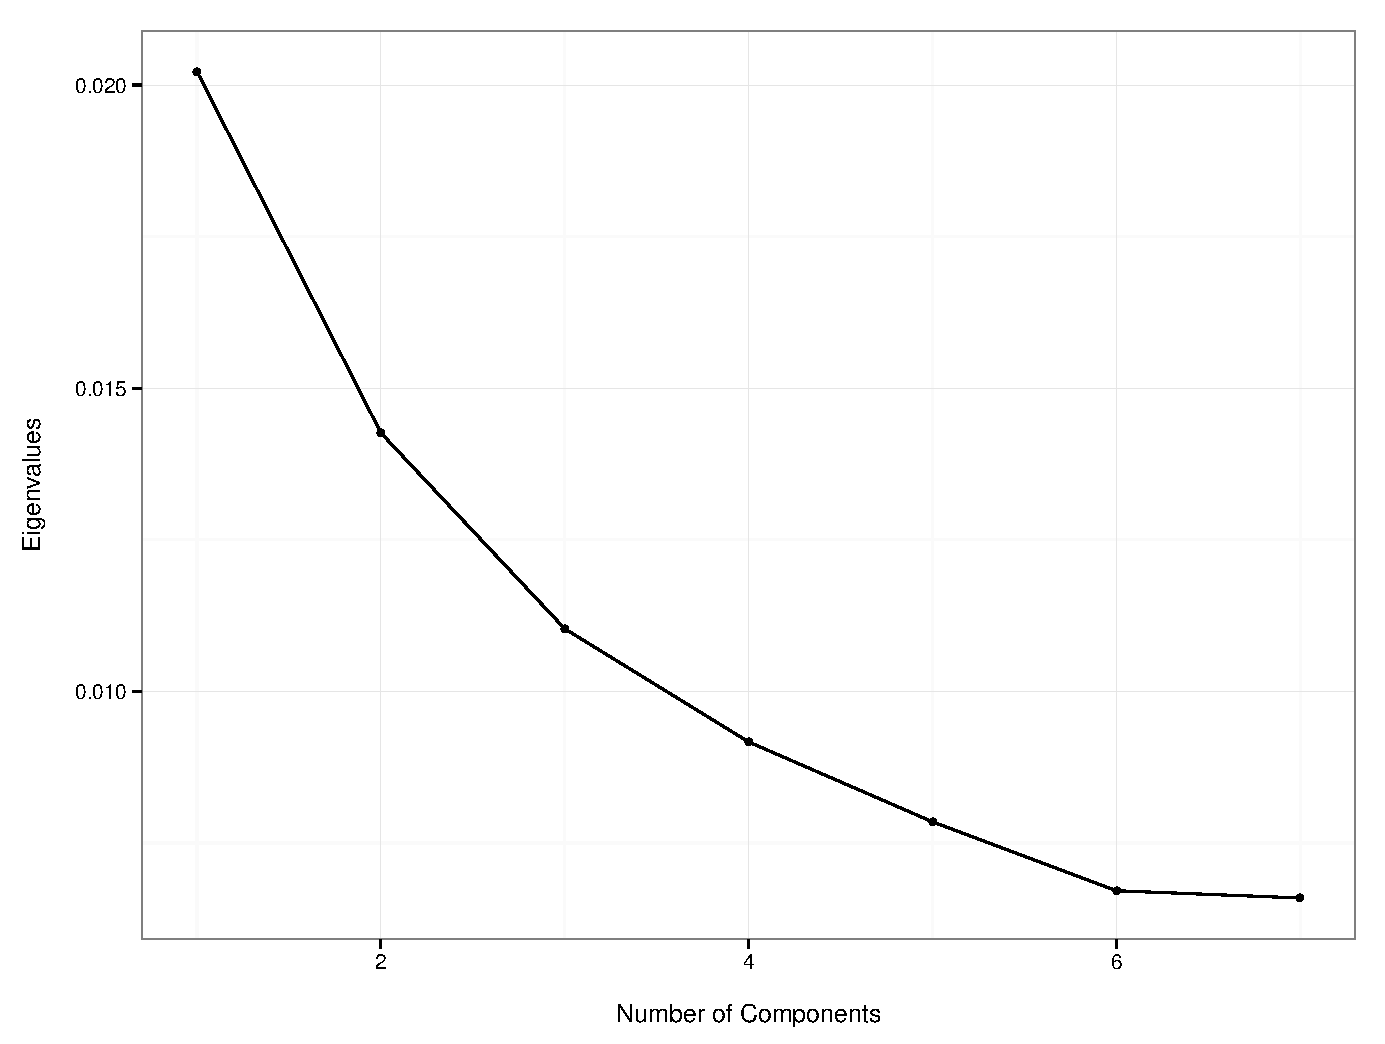
\includegraphics[scale=0.5]{analysis/figures/scree_plot.pdf}
    \end{center}
\end{figure}

\section{Results}\label{results}

The lines in figures \ref{compare_1} and \ref{compare_2} show the
results of the kernel PCA analysis for a selection of countries. We use
the first principal component throughout the paper. Similar plots for
all countries in the analysis are available in the Appendix. Before
diving deeper into these results, it is important to note three simple
transformations we conducted on the raw results. First, we flipped the
scale. As we demonstrate when we compare the Index to other measures of
crisis, this allows higher values of the EPFMS to be interpreted as
`more financial market stress'. Second, we rescaled the Index so that it
would be between zero and one.\footnote{\(\frac{x - \mathrm{min}(\bm{X})}{\mathrm{max}(\bm{X}) - \mathrm{min}(\bm{X})}\),
  where \(\bm{X}\) is the vector of the first principal component and
  \(x\) is an individual value from this vector.} This eases
interpretation and comparability to other measures. Henceforth we only
use the rescaled version of the Index. Then we slightly smoothed the
results by taking a two period--usually two months--moving average.

What does this dimension represent? We took a number of approaches to
answer this question. First, following Spirling (2012) we used a random
forest regression (Breiman 2001; Jones and Linder 2015) to examine the
relationships between word stems from the texts and the Perceptions
Index. Second, we compared the Index to previous indices using an
`interocular' test, e.g.~looking a plots of the results and comparing
them to our priors on financial market stress.

\subsection{Random forest}\label{random-forest}

Spirling (2012, 6--8) demonstrated the usefulness of using random forest
``regressions'' to explore what principal components from textual
analyses represent. To do this we first created a document-term
frequency matrix from the stemmed documents. Effectively this is a
\(k \times s\) matrix recording the frequency of each term in \(\bm{S}\)
for each document in \(\bm{K}\). We removed sparse terms, i.e.~kept only
stems that were found in 90 percent of the documents. Random forest
regressions as opposed to ordinary least squares regressions are useful
in this context because there are many variables--in this case {[}GET{]}
stems--relative to the number of documents--12,482 {[}UPDATE{]}. The
result of this analysis\footnote{We conducted the random forest
  regressions using the \texttt{rfsrc} function from the
  \textbf{randomForestSRC} R package (Ishwaran and Kogalur 2015).} that
we focus on is variable importance shown in Figure \ref{rf_importance}.

\begin{figure}
    \caption{40 Stems Estimated to be the Most Important for Predicting EIU Perception of Financial Market Stress Index}
    \label{rf_importance}

    \begin{center}
        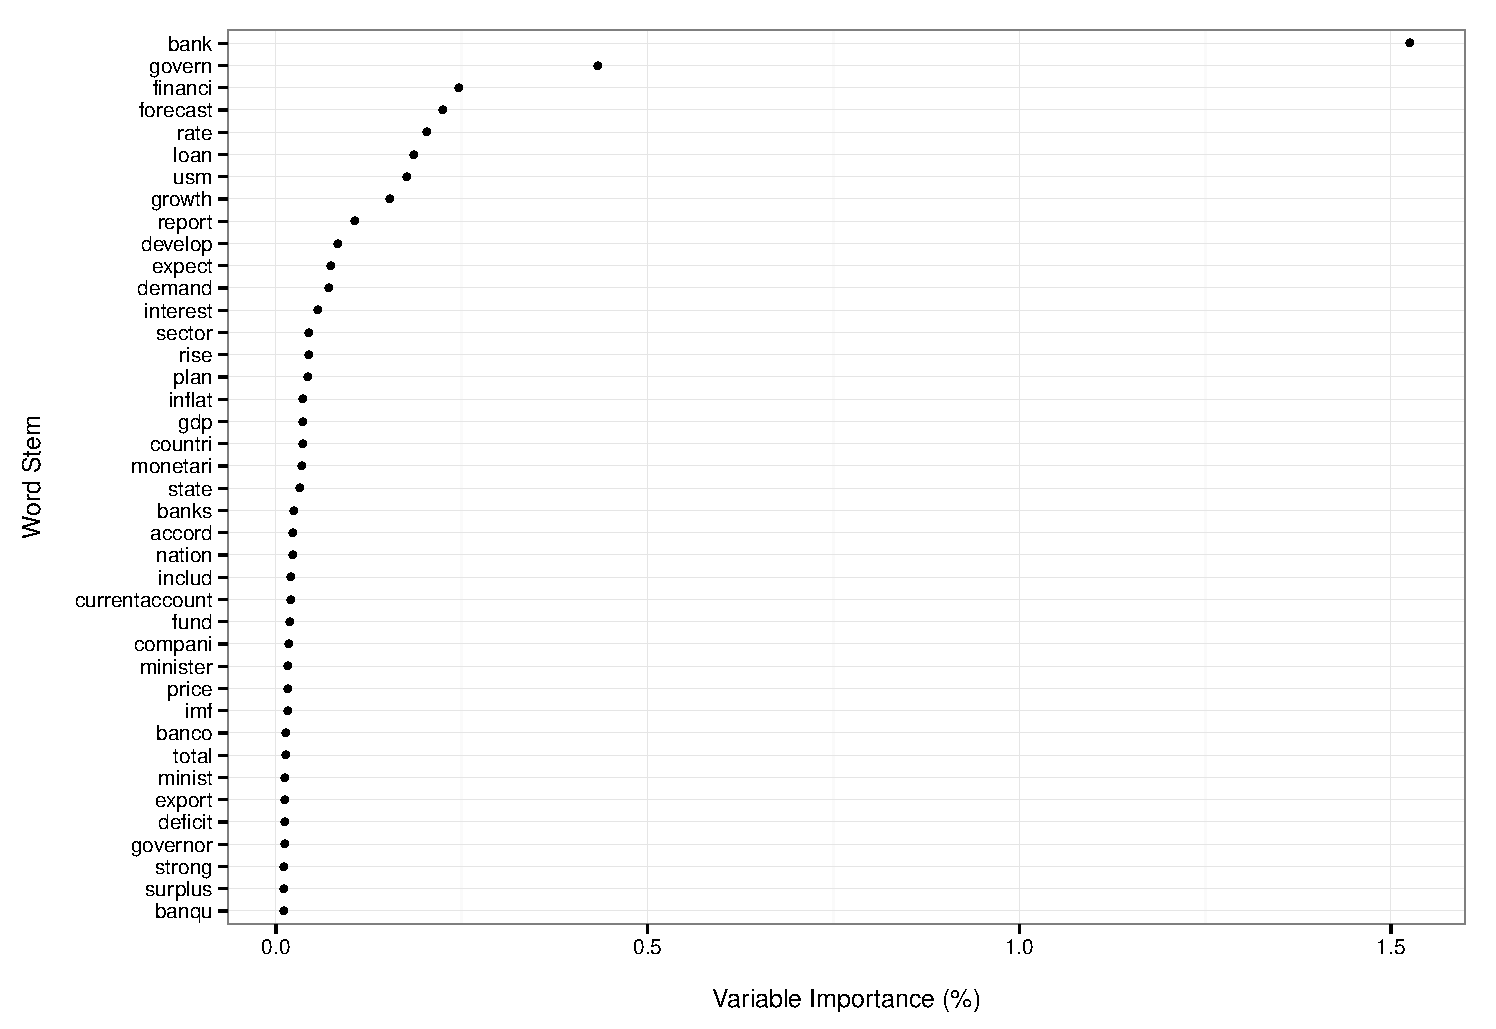
\includegraphics[scale=0.5]{analysis/figures/rf_stem_importance.pdf}
    \end{center}

\end{figure}

\subsection{Comparison to other crisis
measures}\label{comparison-to-other-crisis-measures}

How does our measure compare to previous ways of measuring and timing
financial market stress and crisis? We directly compare our measure to
dichotomous measures in Reinhart and Rogoff (2009) and Laeven and
Valencia (2013) as well as Romer and Romer's (2015) continuous measure.

There are some limitations in comparability based simply on the
different coverage of the different indices. C. Romer and Romer (2015)
in particular largely does not include the most recent crisis in their
sample as they did not collect data past 2007. We had to make a number
of transformations and assumptions to be able to compare the different
data sets. First, the Laeven and Valencia and Reinhart and Rogoff data
on recorded only at yearly intervals. So, we assumed that the crisis
start and end dates they referred to were in the middle of the year,
i.e.~June. Second, we rescaled Romer and Romer's 15-point scale (in
effect 13-points because they do not classify any country-quarter in
their sample as being at the upper two positions on the scale) to be
between 0 and 1 using the same method as above. Finally, it should be
noted that Reinhart and Rogoff (2009) only cover 70 countries and they
have updated their data least recently.

The solid lines in figures \ref{compare_1} and \ref{compare_2} show the
EIU Perceptions of Financial Market Stress Index. The dashed lines show
Romer and Romer's (rescaled) measure. Finally, the shaded boxes show the
periods where Laeven and Valencia (2013) and Reinhart and Rogoff (2009)
classify there as being a banking crisis.\footnote{We used Table 1 in C.
  Romer and Romer (2015) to recreate their data set. We downloaded
  Laeven and Valencia's data from:
  \url{https://www.imf.org/external/pubs/cat/longres.aspx?sk=26015.0}.
  Accessed May 2015. Reinhart and Rogoff's data was downloaded from:
  \url{http://www.carmenreinhart.com/data/browse-by-topic/topics/7/}.
  Accessed May 2015.}

In many cases--given the time period limitations of each data series--,
the indices are roughly congruent. Comparisons with C. Romer and Romer
(2015) are limited, but we can see that in general, where comparable
time series are available, that the EPFMS and their index are roughly
similar. In particular, both indices increase in the US from early 2007.
They both decline for Japan through 2004-2005. A notable difference is
how Romer and Romer classify Japan as being without stress from
mid-2005, while the EPFMS stays high relative to many other economically
developed countries. While they both classify Iceland as being under
stress in the late 2000s, the timing is markedly different. Romer and
Romer classify Iceland as in stress\footnote{They classify Iceland as
  being in a ``minor crisis'' in the second half of 2006 and a ``credit
  disruption'' in the first half of 2007.} in 2006-2007. This is earlier
than not only a marked increase in the EPFMS Index, but also Reinhart
and Rogoff and Laeven and Valencia's timing.

A notable difference between the data series is for Russian. Reinhart
and Rogoff and Laeven and Valencia both record a crisis in the late
2000s, though their timing differ slightly. However, there is no
noticeable change in the EPFMS during this period. This suggests that
perceptions of Russian financial markets in real-time EIU documents did
not noticeably indicate a change in conditions. {[}CHECK WHEN RESULTS
ARE UPDATED{]}

Overall, the similarities between EPFMS scores and other measures of
banking crises suggests that the EPFMS Index does capture aspects of
financial market stress. In particular, higher values of the EPFMS are
indicate higher levels of perceived financial market stress. At the same
time, the differences between the measures also indicates that the EPFMS
sheds unique light on processes not captured well by previous indices.
One major difference that we will now look at in more detail is how
having a continuous indicator allows us to consider how levels perceived
financial market stress differ between developed and developing
countries.

\begin{figure}
    \caption{Comparing Perceptions of Financial Market Conditions to Laeven \& Valencia (2012) and Reinhart \& Rogoff (2009) (1)}
    \label{compare_1}
    \begin{center}
        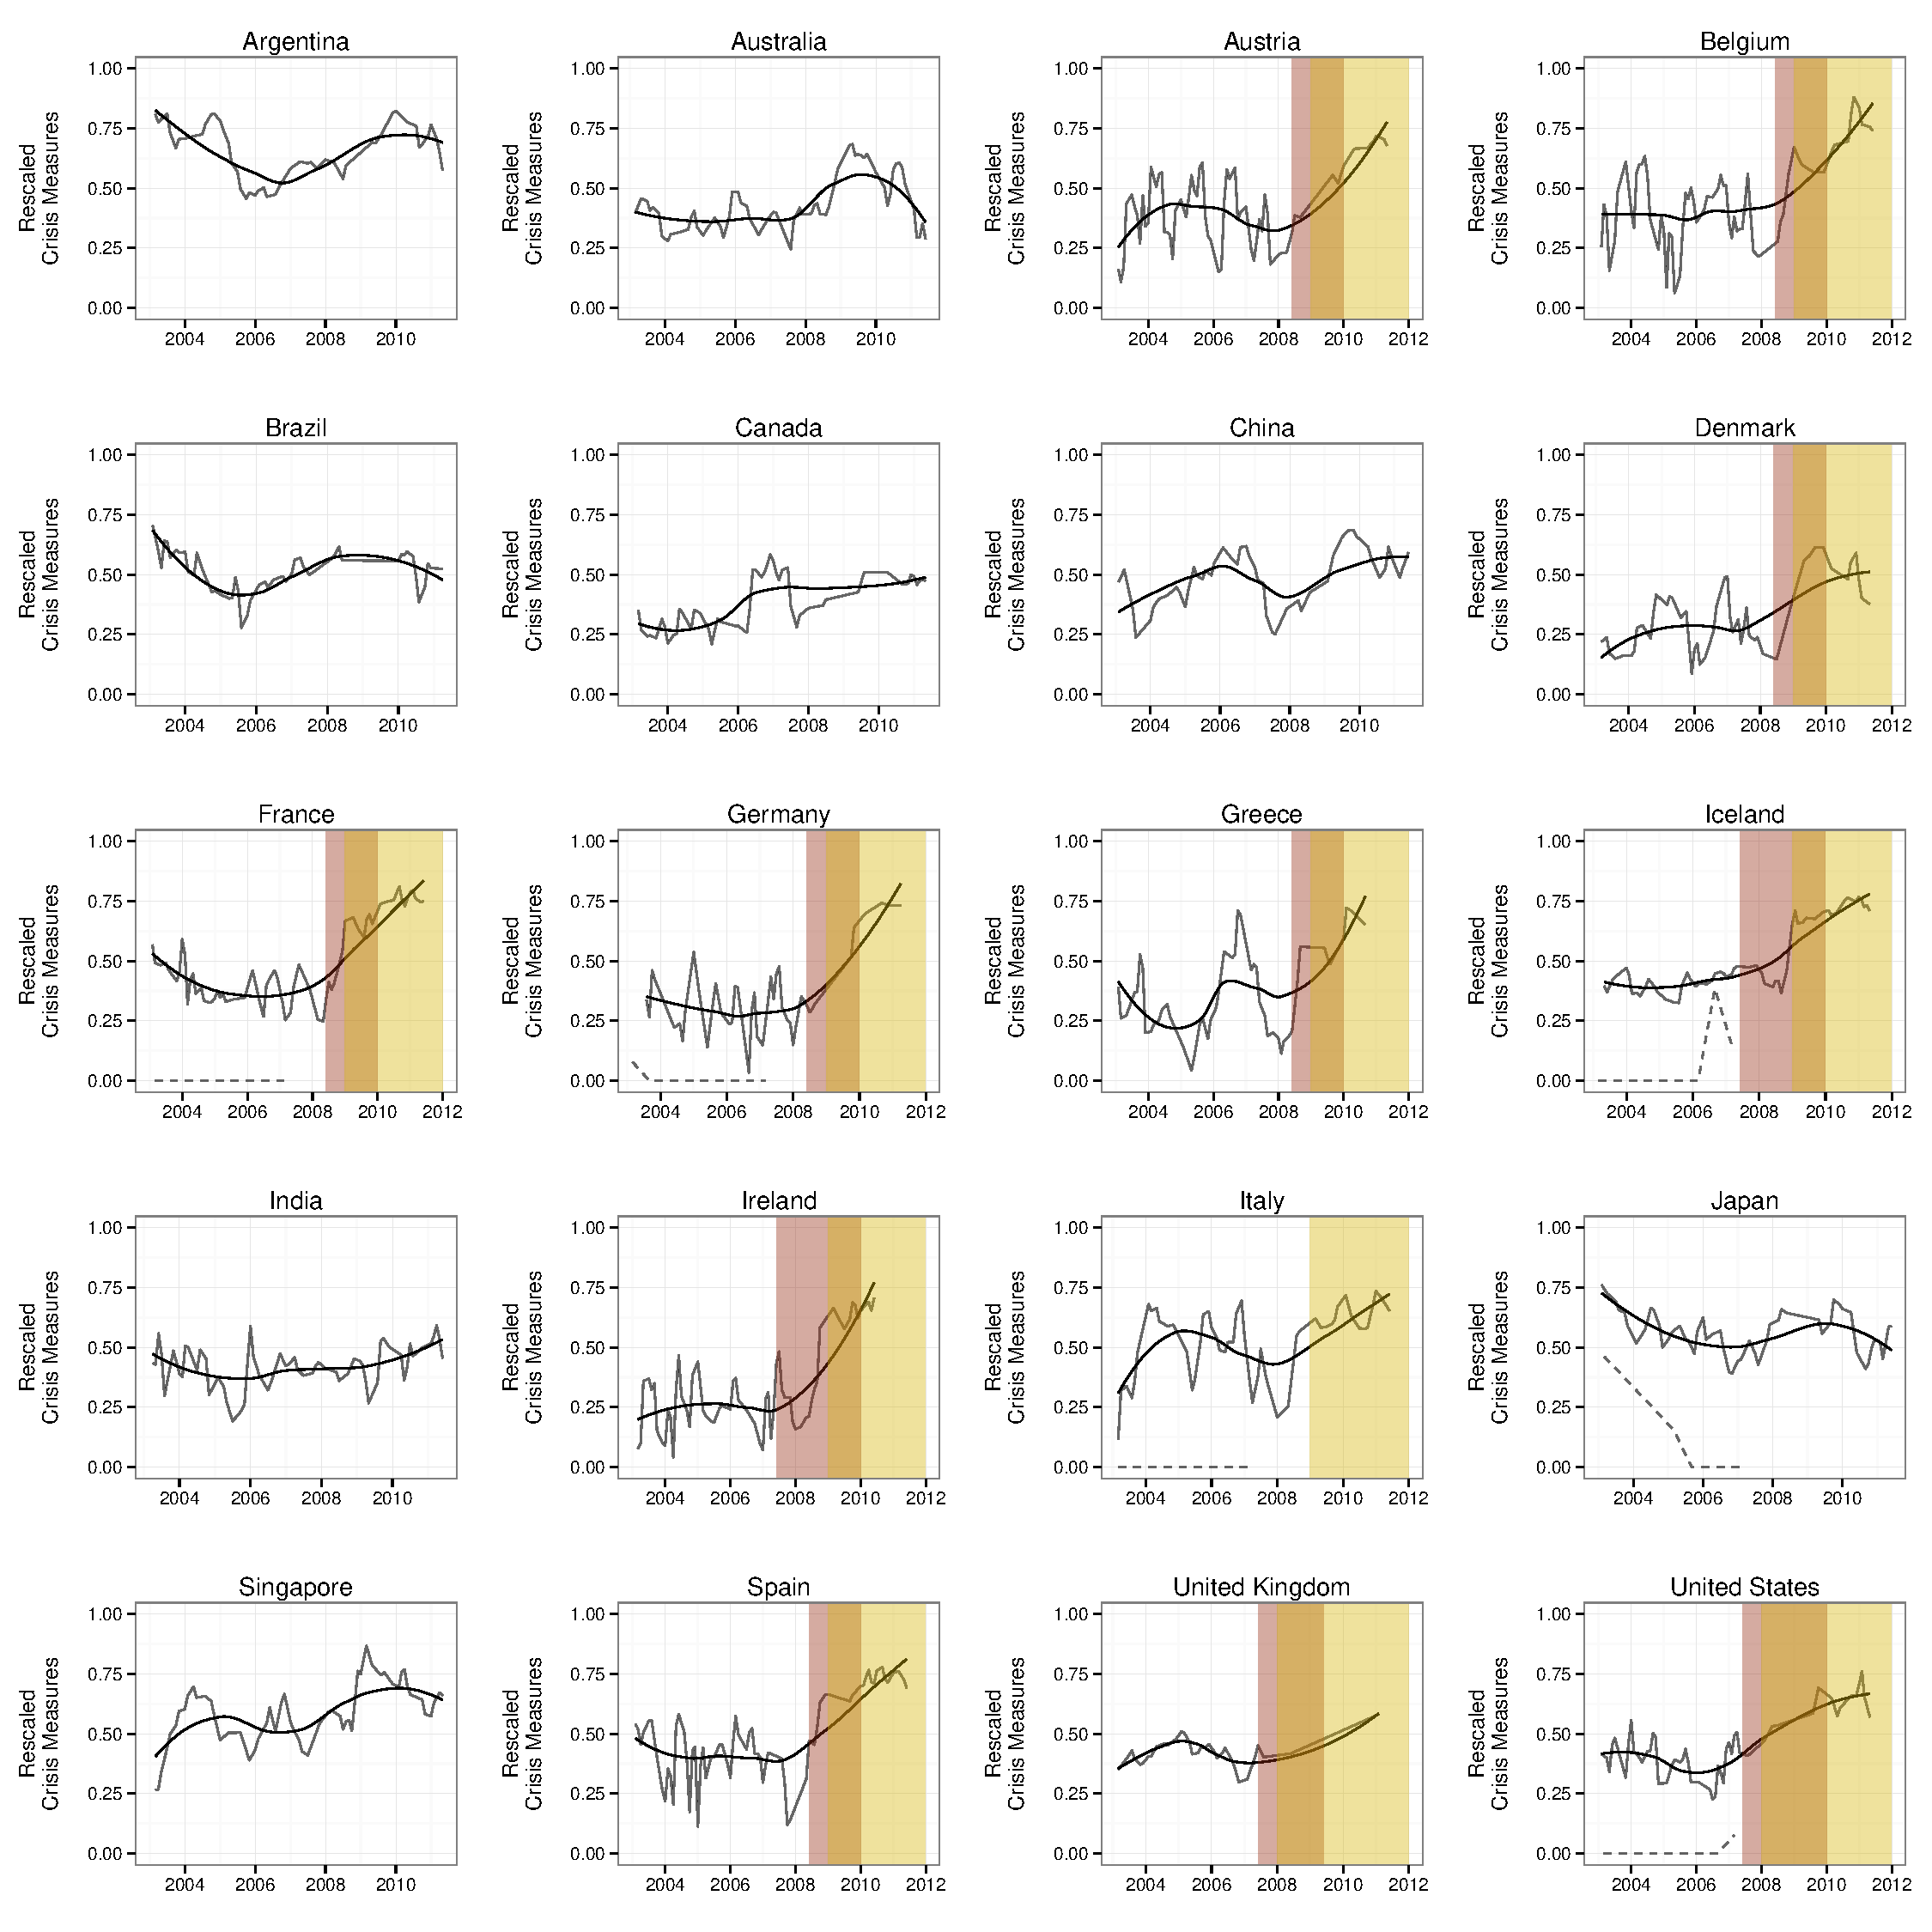
\includegraphics[scale=0.4]{analysis/figures/compare_to_lv_rr.pdf}
    \end{center}

    {\tiny{Solid lines show the (rescaled) EIU Perceptions of Financial Market Stress indicator. Dotted lines represent a loess smooth of these series. \\

    Dashed lines show Romer and Romer's (2015) rescaled index. \\

    Yellow shaded areas indicate periods that Laeven and Valencia (2012) classify as systemic banking crises. Note that crises are automatically terminated at the end of 2011 due to the series not extending beyond this point, not necessarily because the crisis finished. \\

    Red shaded areas indicate periods that Reinhart and Rogoff (2009) classify as banking crises. Note that crises are automatically terminated at the end of 2009 due to the series not extending beyond this point, not necessarily because the crisis finished. \\

    Orange areas indicate periods where a crisis is recorded for both measures.}}
\end{figure}

\begin{figure}
    \caption{Comparing Perceptions of Financial Market Conditions to Laeven \& Valencia (2012) and Reinhart \& Rogoff (2009) (2)}
    \label{compare_2}
    \begin{center}
        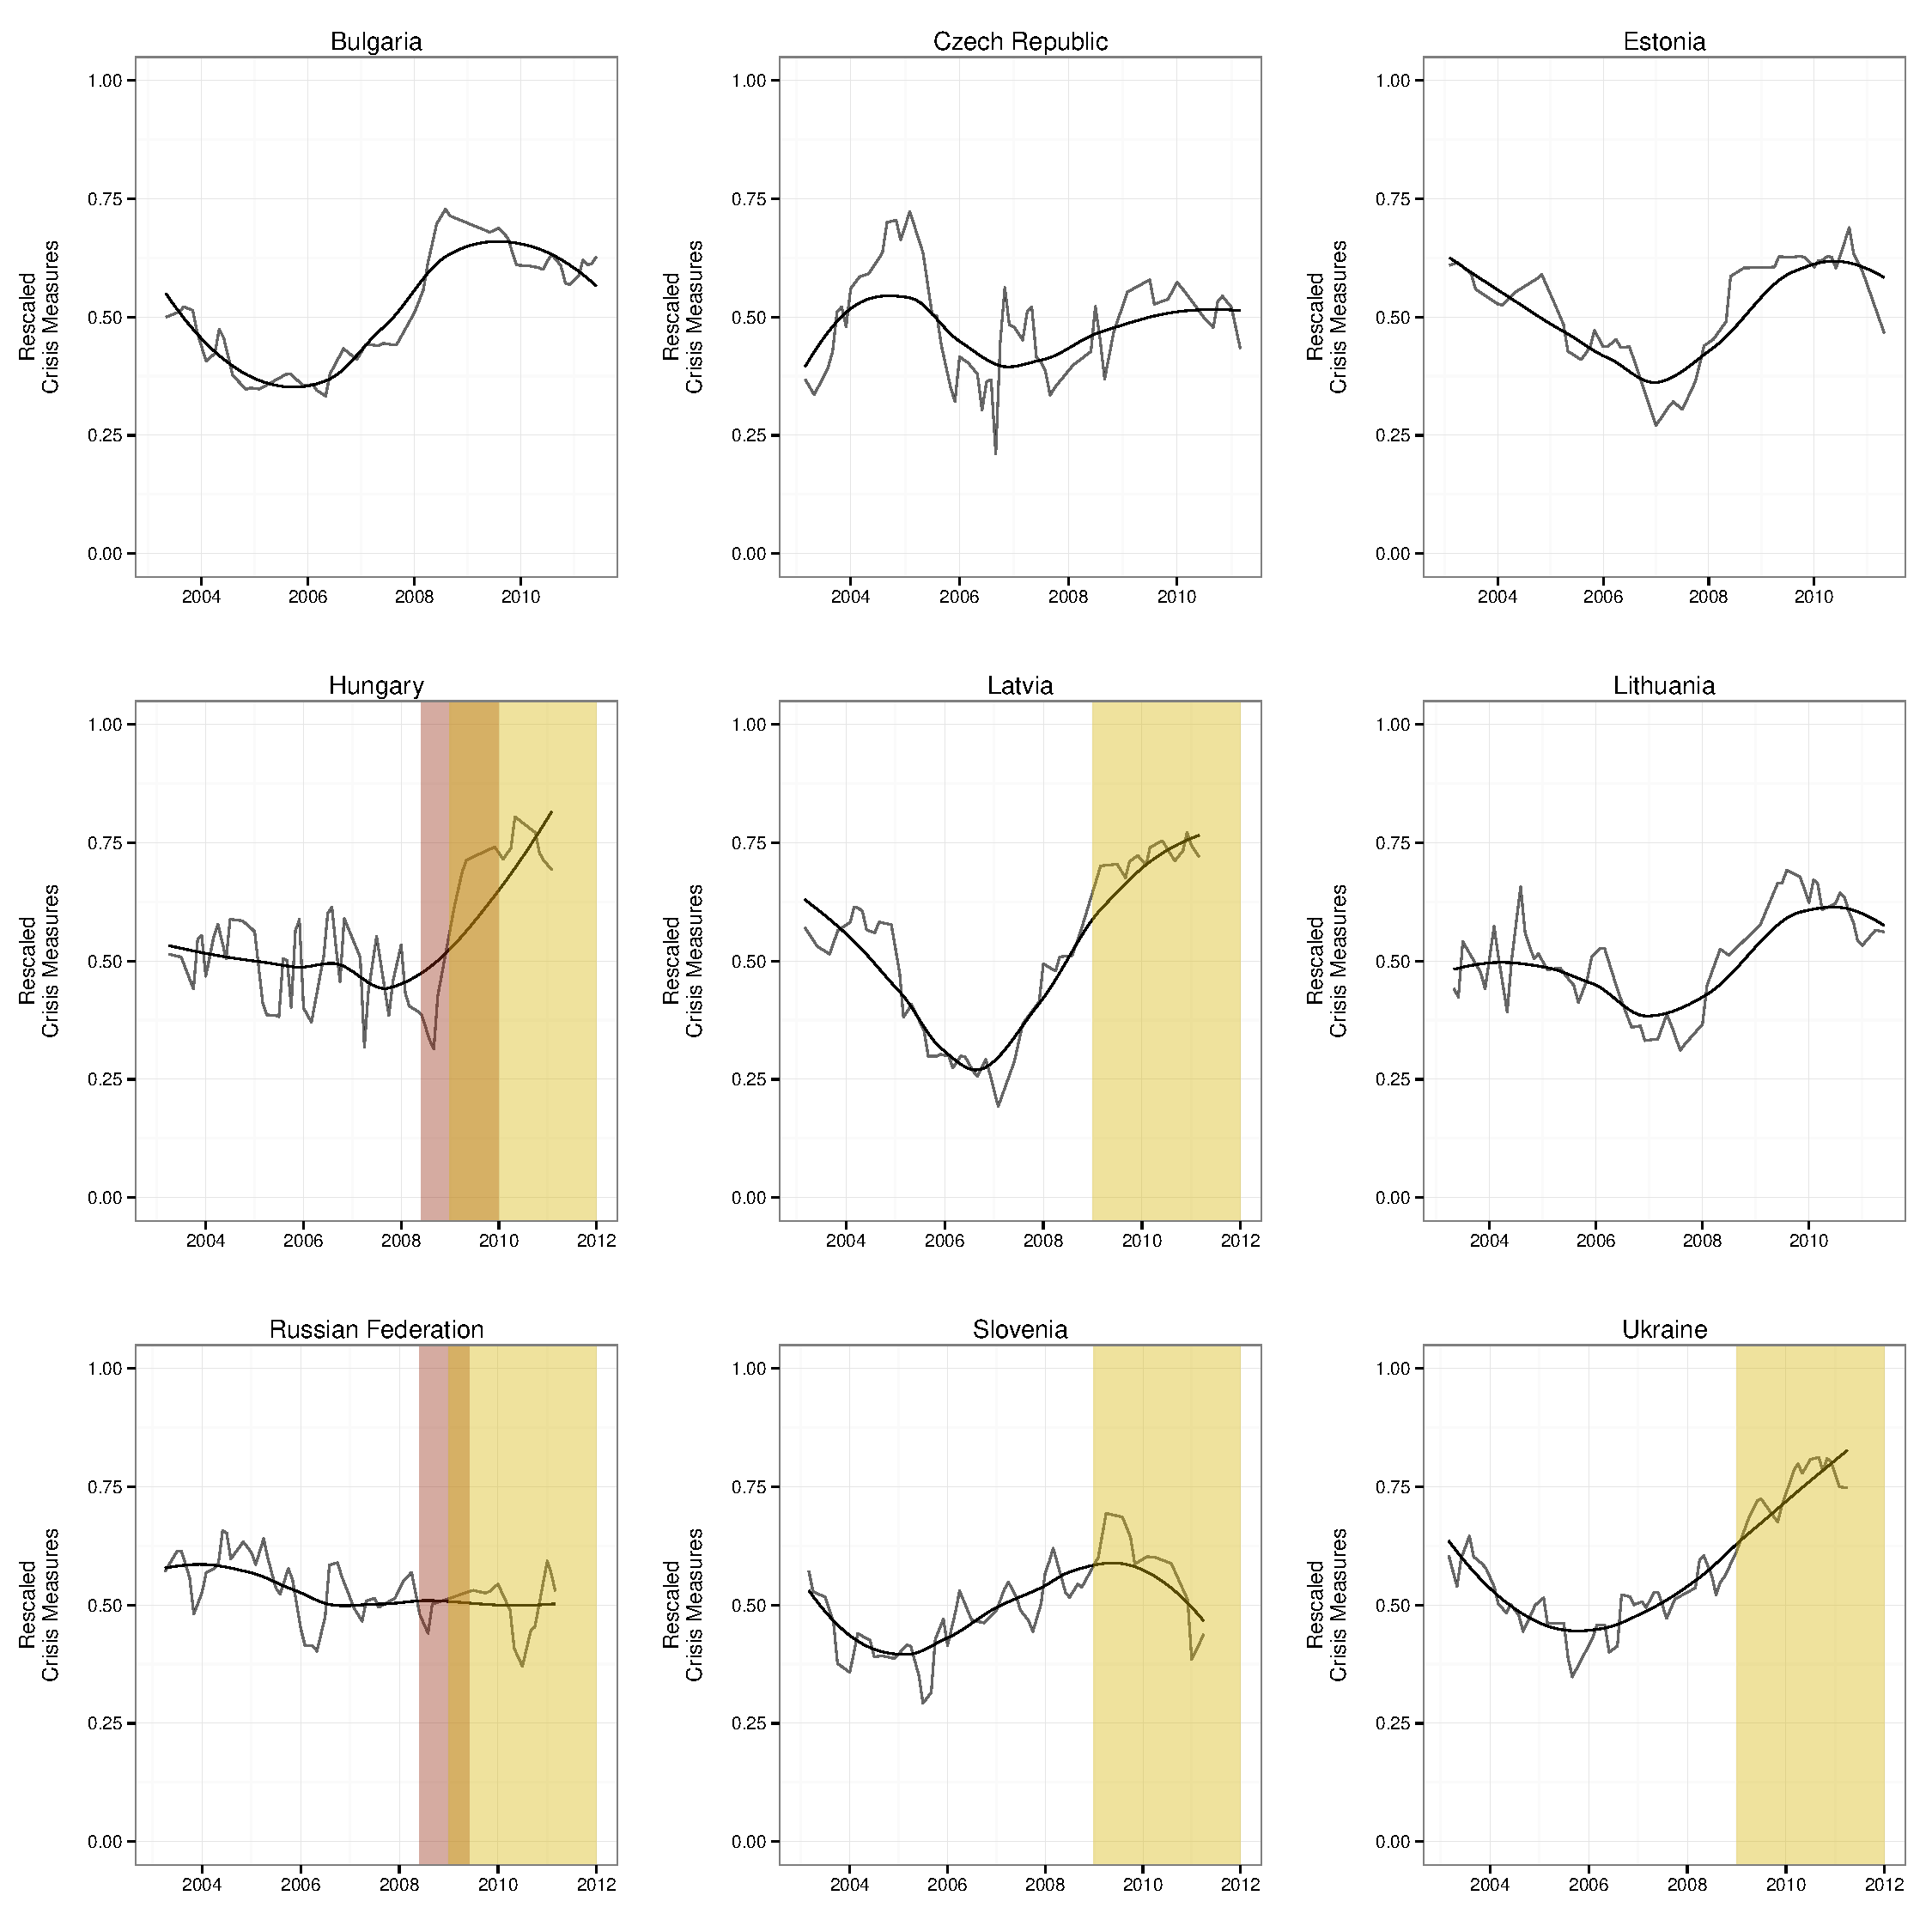
\includegraphics[scale=0.4]{analysis/figures/compare_to_lv_rr_2.pdf}
    \end{center}

    {\tiny{Solid lines show the (rescaled) EIU Perceptions of Financial Market Stress indicator. Dotted lines represent a loess smooth of these series. \\

    Yellow shaded areas indicate periods that Laeven and Valencia (2012) classify as systemic banking crises. Note that crises are automatically terminated at the end of 2011 due to the series not extending beyond this point, not necessarily because the crisis finished. \\

    Red shaded areas indicate periods that Reinhart and Rogoff (2009) classify as banking crises. Note that crises are automatically terminated at the end of 2009 due to the series not extending beyond this point, not necessarily because the crisis finished. \\

    Orange areas indicate periods where a crisis is recorded for both measures.}}
\end{figure}

\subsection{Developed vs.~Developing
countries}\label{developed-vs.developing-countries}

An important finding from examining the Index is that there is a clear
difference in the level of perceived financial market stress in
developed and developing countries. Notably, developing countries often
have scores well above 0.5, while many developed countries only reach
this level during financial crises. Developing countries often lack
strong financial institutions and systems {[}CITE{]}, so we should
expect them to face generally tighter credit market conditions than
developed countries. Formal financial markets are less important for
developing countries' economies {[}CITE{]}.

These observations should lead to an important refinement to how the
Index should be interpreted and how it should be used in empirical work.
First, the Index measures banking market conditions, but not ``crisis''
directly. Instead, perceived crisis is likely the result of an
interaction between the Index and the importance of financial markets
for sustaining a country's economy. Though policy-makers in developing
economies face generally tight credit market conditions, these
persistent conditions likely do not threaten the wider \emph{status quo}
economy. As such, we would not expect significant policy responses to
address financial market stress in these places. Conversely, tightening
of credit market conditions in a developed, financialized economy would
likely have large negative implications for the wider economy. So, we
would expect these politicians to respond to worsening credit market
conditions.

Previous measures of financial market distress and crises have generally
been unable to explore this possible interaction. \emph{Post-hoc}
measures of crisis in particular capture the outcome of this process,
rather than the process itself.

\section{Replication}\label{replication}

\section{Conclusions and Possible Future
Work}\label{conclusions-and-possible-future-work}

\section{Appendix}\label{appendix}

\section*{References}\label{references}
\addcontentsline{toc}{section}{References}

Breiman, Leo. 2001. ``Random Forests.'' \emph{Machine Learning} 45 (1):
5--32.

Chaudron, Raymond, and Jakob de Haan. 2014. ``Dating Banking Crises
Using Incidence and Size of Bank Failures: Four Crises Reconsidered.''
\emph{Journal of Financial Stability}, 1--34.

Copelovitch, Mark, Christopher Gandrud, and Mark Hallerberg. 2015.
``Financial Regulatory Transparency, International Institutions, and
Borrowing Costs.'' \emph{Working Paper}.

Feinerer, Ingo, and Kurt Hornik. 2015. \emph{tm: Text Mining Package}.
\url{http://CRAN.R-project.org/package=tm}.

Gandrud, Christopher, and Mark Hallerberg. 2015. ``When All Is Said and
Done: Updating 'Elections, Special Interests, and Financial Crisis'.''
\emph{Research and Politics}.

Grimmer, Justin, and Brandon M Stewart. 2013. ``Text as Data: The
Promise and Pitfalls of Automatic Content Analysis Methods for Political
Texts.'' \emph{Political Analysis} 21 (3): 267--97.

Ishwaran, H., and U.B. Kogalur. 2015. \emph{Random Forests for Survival,
Regression and Classification (RF-SRC)}. manual.
\url{http://cran.r-project.org/web/packages/randomForestSRC/}.

Jing, Zhongbo, Jakob de Haan, Jan Jacobs, and Haizhen Yang. 2015.
``Identifying Banking Crises Using Money Market Pressure: New Evidence
for a Large Set of Countries.'' \emph{Journal of Macroeconomics} 43 (C):
1--20.

Jones, Zachary, and Fridolin Linder. 2015. ``Exploratory Data Analysis
Using Random Forests.'' \emph{Paper Presented at the Annual MPSA
Conference}.

Karatzoglou, Alexandros, Alex Smola, Kurt Hornik, and Achim Zeileis.
2004. ``kernlab -- an S4 Package for Kernel Methods in R.''
\emph{Journal of Statistical Software} 11 (9): 1--20.
\url{http://www.jstatsoft.org/v11/i09/}.

Laeven, Luc, and Fabi{á}n Valencia. 2013. ``Systemic Banking Crisis
Database.'' \emph{IMF Economic Review} 61 (2): 225--70.

Lodhi, Huma, Craig Saunders, John Shawe-Taylor, Nello Cristianini, and
Chris Watkins. 2002. ``Text Classification Using String Kernels.''
\emph{The Journal of Machine Learning Research} 2. JMLR. org: 419--44.

R Core Team. 2015. \emph{R: A Language and Environment for Statistical
Computing}. Vienna, Austria: R Foundation for Statistical Computing.
\url{http://www.R-project.org/}.

Reinhart, Carmen, and Kenneth Rogoff. 2009. \emph{This Time Is
Different: Eight Centuries of Financial Folly}. Princeton: Princeton
University Press.

Romer, Christina, and David Romer. 2015. ``New Evidence on the Impact of
Financial Crises in Advanced Countries,'' April, 1--65.

Rosas, Guillermo. 2009. ``Dynamic Latent Trait Models: An Application to
Latin American Banking Crises.'' \emph{Electoral Studies} 28: 375--87.

Scholkopf, B., A. Smola, and K. Muller. 1998. ``Nonlinear Component
Analysis as a Kernel Eigenvalue Problem.'' \emph{Neural Computation} 10:
1299--1319.

Spirling, Arthur. 2012. ``U.S. Treaty Making with American Indians:
Institutional Change and Relative Power, 1784-1911.'' \emph{American
Journal of Political Science} 56 (1): 84--97.

{Von Hagen}, Jorgen, and T. Ho. 2007. ``Money Market Pressure and the
Determinants of Banking Crises.'' \emph{Journal of Money, Credit, and
Banking} 39 (5): 1037--66.

Zhang, Rui, Wenjian Wang, and Yichen Ma. 2010. ``Approximations of the
Standard Principal Components Analysis and Kernel PCA.'' \emph{Expert
Systems with Applications} 37 (9): 6531--37.

\end{document}
